%
% $RCSfile: paradigm_overview.tex,v $
%
% Copyright (C) 2002-2008. Christian Heller.
%
% Permission is granted to copy, distribute and/or modify this document
% under the terms of the GNU Free Documentation License, Version 1.1 or
% any later version published by the Free Software Foundation; with no
% Invariant Sections, with no Front-Cover Texts and with no Back-Cover
% Texts. A copy of the license is included in the section entitled
% "GNU Free Documentation License".
%
% http://www.cybop.net
% - Cybernetics Oriented Programming -
%
% http://www.resmedicinae.org
% - Information in Medicine -
%
% Version: $Revision: 1.1 $ $Date: 2008-08-19 20:41:08 $ $Author: christian $
% Authors: Christian Heller <christian.heller@tuxtax.de>
%

\subsection{Paradigm Overview}
\label{paradigm_overview_heading}
\index{Paradigm Overview}
\index{Programming Paradigm Systematics}
\index{Imperative (Command Oriented) Programming Language}
\index{Declarative Programming Language}
\index{Machine Language}
\index{Assembly Language}
\index{System Programming}
\index{Functional Programming}
\index{Logical Programming}
\index{Scripting Language}
\index{Typeless Programming}
\index{Structured- and Procedural Programming}
\index{SPP}
\index{Object Oriented Programming}
\index{OOP}
\index{Programming Paradigms as Contrasting Pairs}

Several other systematics, besides the historical one shown in the previous
section, exist to categorise programming languages and their paradigms. Some
authors, for example, divide computer languages into those that have to be
compiled before being executed and those which are interpreted at runtime.
Figure \ref{paradigm_figure} shows yet another arbitrary, tree-like systematics
that was assembled on the basis of \cite{wikipedia} and \cite{kinnersley}.

\begin{figure}[ht]
    \begin{center}
        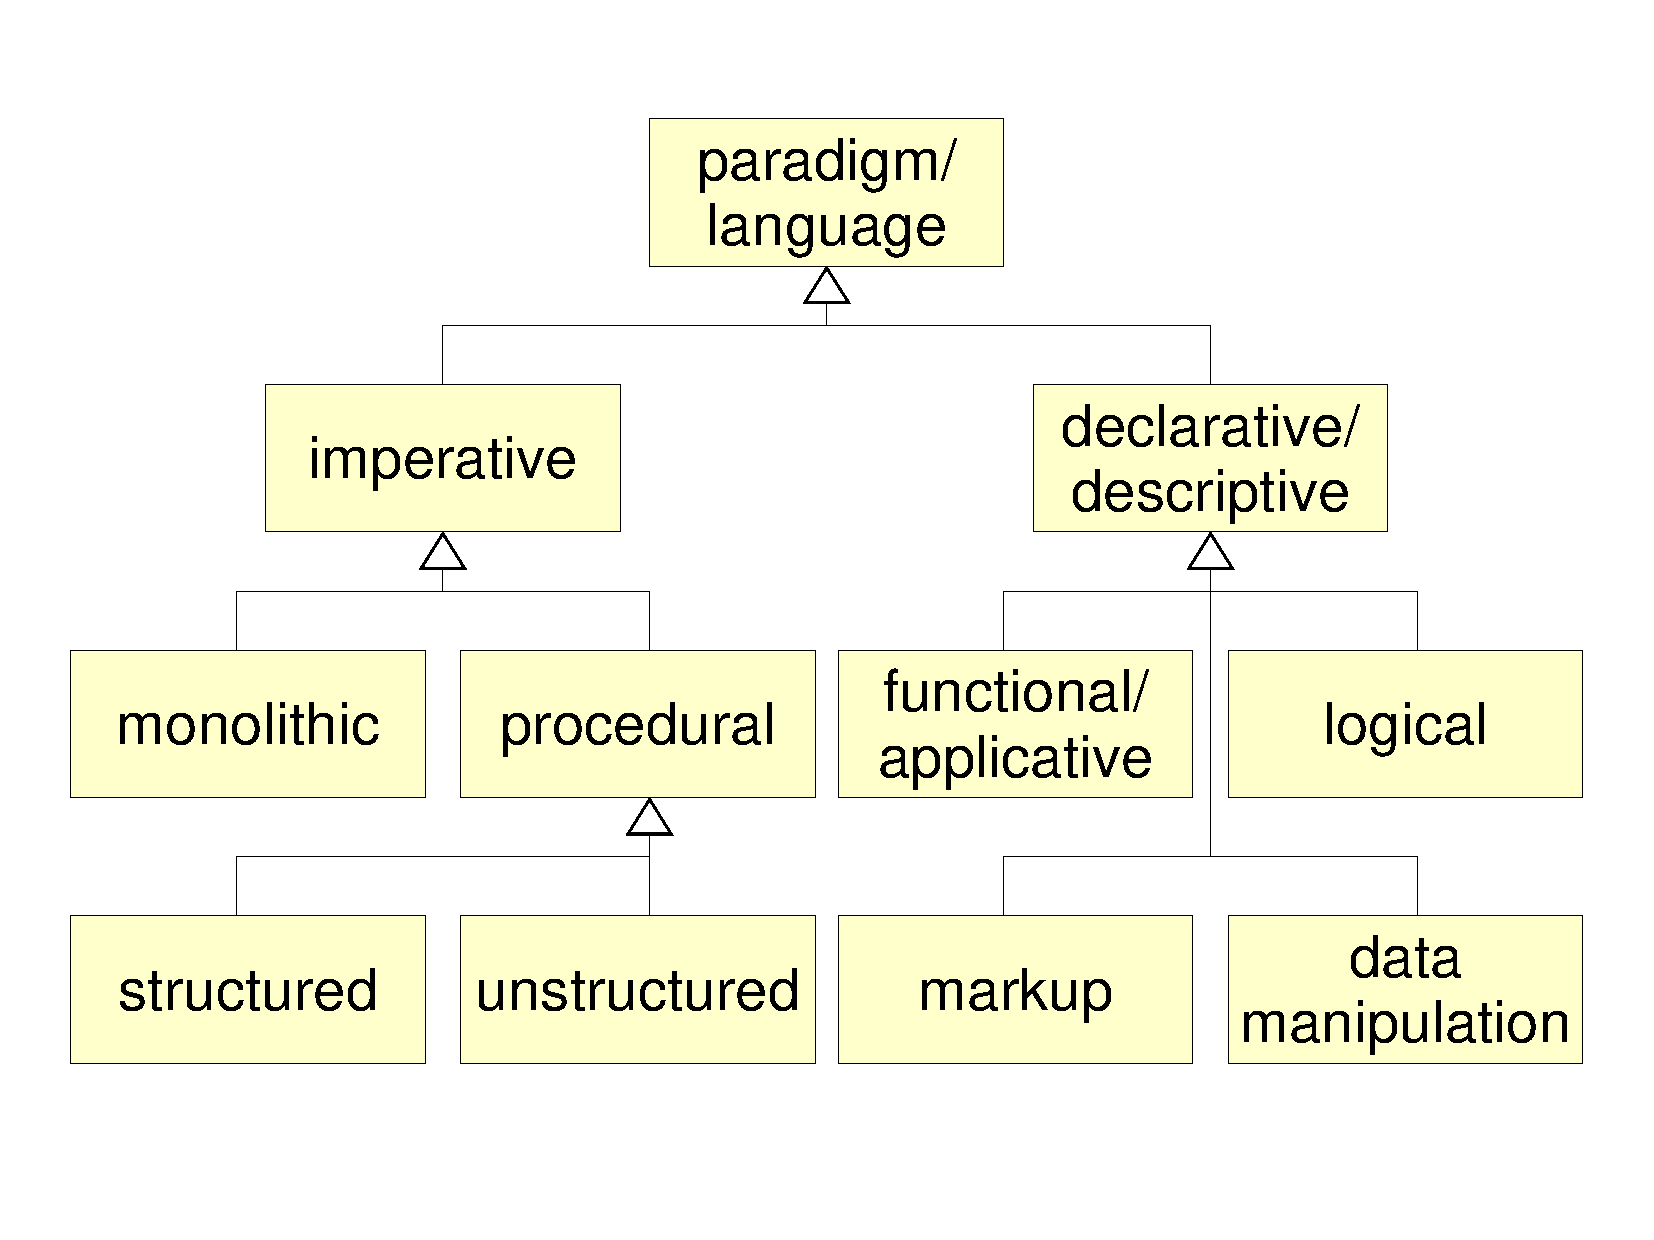
\includegraphics[scale=0.3,angle=-90]{graphic/paradigm.pdf}
        \caption{Programming Paradigm Systematics}
        \label{paradigm_figure}
    \end{center}
\end{figure}

\emph{Machine-} and \emph{Assembly Language} as well as \emph{System Programming}
are \emph{imperative} (command-oriented). \emph{Functional-} and
\emph{Logical Programming}, on the other hand, are \emph{declarative}, just as
most \emph{Scripting Languages} used for \emph{Typeless Programming}. The
boundaries tend to be vague, however. Many of the new languages borrow features
from more than one programming paradigm. Similarly, the concepts of
\emph{Structured and Procedural Programming} (SPP) and
\emph{Object Oriented Programming} (OOP) are not only used in system
programming-, but also in scripting languages.

It is important to note that it is extremely difficult, if not impossible, to
arrange all programming languages into just one tree of categories. Kinnersley
\cite{kinnersley} writes that \textit{for every classification scheme there
will be a large proportion of languages that do not fit \ldots\ most languages
are not purely one or the other}. The \emph{Logo} language, for example, is an
adaptation of the functional language \emph{Lisp}, that is non-imperative, yet
procedural \cite{wikipedia}. Figure \ref{paradigm_figure} can therefore only be
seen as trial to create a systematics of the most common programming paradigms.
In order to avoid miscategorisation, the Wikipedia Encyclopedia \cite{wikipedia}
prefers to list programming paradigms as contrasting pairs, for example:

\begin{itemize}
    \item[-] Procedural vs. Functional
    \item[-] Imperative vs. Declarative
    \item[-] Structured vs. Unstructured
    \item[-] Value-level vs. Function-level
    \item[-] Flow-driven vs. Event-driven
    \item[-] Scalar vs. Array
    \item[-] Class-based vs. Prototype-based
    \item[-] Rule-based vs. Constraint
\end{itemize}

Not all items of the list are explained in this work since this would break its
frame and focus. However, some of the most important programming language
concepts in use today are described in the following sections.
